\documentclass{article}
\usepackage{amsmath}
\usepackage{amssymb}
\usepackage{graphicx}
\usepackage{hyperref}
\usepackage[version=4]{mhchem}


\begin{document}
\section*{Problem}
Medians \(B D\) and \(C E\) of a triangle \(A B C\) are perpendicular, \(C E=24\) and the area of triangle \(A B C\) is 288 . Find the length of \(B D\).\\
\centering
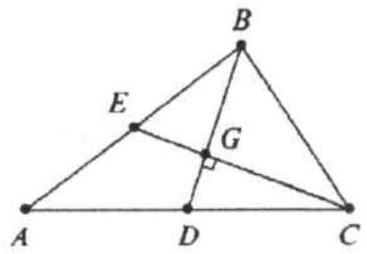
\includegraphics[width=\textwidth]{images/015(2).jpg}

\section*{Solution}
(D).\\
Draw perpendiculars from \(D\) and \(C\) to \(A B\).\\
We observe a \(30^{\circ}-60^{\circ}-90^{\circ}\) right triangle (with the sides \(12,12 \sqrt{3}\), and 24 ) and a \(45^{\circ}-45^{\circ}-90^{\circ}\) right triangle (with the sides \(12,12,12 \sqrt{2}\) ).\\
\centering
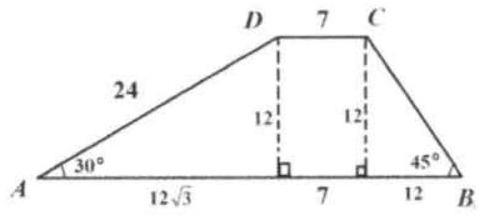
\includegraphics[width=\textwidth]{images/092(2).jpg}

So \(A B=7+12+12 \sqrt{3}=19+12 \sqrt{3}\).

\end{document}
